\documentclass[a4paper,11pt]{article}

\usepackage{fullpage}
\usepackage[usenames,dvipsnames]{color}
\usepackage{hyperref}
\usepackage{amsmath}
\usepackage{amssymb}
\usepackage{tikz}

\usetikzlibrary{positioning}

\hypersetup{
  colorlinks,%
    citecolor=black,%
    filecolor=black,%
    linkcolor=black,%
    urlcolor=mygreylink     % can put red here to visualize the links
}

\newcommand{\Pred}[2]{\ensuremath{\mathtt{Predator}\left<#1, #2\right>}}
\newcommand{\Prey}[2]{\ensuremath{\mathtt{Prey}\left<#1, #2\right>}}
\newcommand{\p}[2]{\ensuremath{\mathtt{P}\left<#1, #2\right>}}

\newcommand{\DrawSmallPred}[2]{\node at (A.center #1 #2) {$\pi$};}
\newcommand{\DrawSmallPrey}[2]{\node at (A.center #1 #2) {P};}
\newcommand{\DrawBigPred}[2]  {\node at (A.center #1 #2) {\Huge $\pi$};}
\newcommand{\DrawBigPrey}[2]  {\node at (A.center #1 #2) {\Huge P};}

\definecolor{mygrey}{gray}{.85}
\definecolor{mygreylink}{gray}{.30}
\textheight=8.6in
\raggedbottom
\raggedright
\setlength{\tabcolsep}{0in}
\addtolength{\oddsidemargin}{-0.375in}
\addtolength{\evensidemargin}{0.375in}
\addtolength{\textwidth}{0.5in}
\addtolength{\topmargin}{-.375in}
\addtolength{\textheight}{0.75in}

% For drawing grids
\makeatletter
\pgfkeys{/pgf/grid lines/.initial=2}

\pgfdeclareshape{grid}{
    % inherit most things from the rectangle shape
    \inheritsavedanchors[from=rectangle]
    \inheritanchorborder[from=rectangle]
    \inheritanchor[from=rectangle]{center}
    \inheritanchor[from=rectangle]{north}
    \inheritanchor[from=rectangle]{south}
    \inheritanchor[from=rectangle]{west}
    \inheritanchor[from=rectangle]{east}
    \inheritanchor[from=rectangle]{south east}
    \inheritanchor[from=rectangle]{south west}
    \inheritanchor[from=rectangle]{north east}
    \inheritanchor[from=rectangle]{north west}
    \inheritbackgroundpath[from=rectangle]

    \savedmacro\lines{%
        \pgfmathtruncatemacro\lines{\pgfkeysvalueof{/pgf/grid lines}}%
    }

    % draw the grid
    \beforebackgroundpath{
        % store lower right in xa/ya and upper right in xb/yb
        \southwest \pgf@xa=\pgf@x \pgf@ya=\pgf@y
        \northeast \pgf@xb=\pgf@x \pgf@yb=\pgf@y

        % compute distance between the lines
        \pgfmathparse{(\the\pgf@xb-\the\pgf@xa)/(\lines + 1)}
        \pgf@xc=\pgfmathresult pt
        \pgfmathparse{(\the\pgf@yb-\the\pgf@ya)/(\lines + 1)}
        \pgf@yc=\pgfmathresult pt

        % draw grid
        \c@pgf@counta=0
        \c@pgf@countb\lines\relax
        \pgf@xb=\pgf@xa
        \advance\pgf@xb\pgf@xc\relax
        \pgfmathloop
            \ifnum\c@pgf@counta<\c@pgf@countb
                \pgfpathmoveto{\pgfpoint{\pgf@xb}{\pgf@ya}}
                \pgfpathlineto{\pgfpoint{\pgf@xb}{\pgf@yb}}
                \advance\c@pgf@counta 1\relax
                \advance\pgf@xb\pgf@xc\relax
        \repeatpgfmathloop
        % set \pgf@xb to the right side
        \c@pgf@counta=0
        \pgf@yb=\pgf@ya
        \advance\pgf@yb\pgf@yc\relax
        \pgfmathloop
            \ifnum\c@pgf@counta<\c@pgf@countb
                \pgfpathmoveto{\pgfpoint{\pgf@xa}{\pgf@yb}}
                \pgfpathlineto{\pgfpoint{\pgf@xb}{\pgf@yb}}
                \advance\c@pgf@counta 1\relax
                \advance\pgf@yb\pgf@yc\relax
        \repeatpgfmathloop
        \pgfusepath{stroke}
    }

    % add anchors for vertices (intersections of grid lines)
    % and center points (centers of the small rectangles).
    %
    % vertex anchors are simply called 'x y' with '0 0' being the lower left
    % vertex.
    % center anchors are called 'center x y' with 'center 1 1' being the center
    % of the lower left rectangle
    \pgfutil@g@addto@macro\pgf@sh@s@grid{%
        \c@pgf@counta\lines
        \advance\c@pgf@counta 1\relax
        \pgfmathloop\ifnum\c@pgf@counta>-1
            {% group to allow nesting of loops
                \c@pgf@countb\lines
                \advance\c@pgf@countb 1\relax
                \pgfmathloop\ifnum\c@pgf@countb>-1
                    \pgfutil@ifundefined{pgf@anchor@grid@\the\c@pgf@counta\space\the\c@pgf@countb}{%
                        % need to use xdef, so that \c@pgf@counta/b are expanded
                        % vertices
                        \expandafter\xdef\csname pgf@anchor@grid@\the\c@pgf@counta\space\the\c@pgf@countb\endcsname{%
                            \noexpand\southwest \noexpand\pgf@xa=\noexpand\pgf@x \noexpand\pgf@ya=\noexpand\pgf@y
                            \noexpand\northeast \noexpand\pgf@xb=\noexpand\pgf@x \noexpand\pgf@yb=\noexpand\pgf@y
                            \noexpand\pgfmathparse{(\noexpand\the\noexpand\pgf@xb-\noexpand\the\noexpand\pgf@xa)/(\noexpand\lines + 1)*\the\c@pgf@counta}
                            \noexpand\pgf@x=\noexpand\pgf@xa\noexpand\relax
                            \noexpand\advance\noexpand\pgf@x\noexpand\pgfmathresult pt\noexpand\relax
                            \noexpand\pgfmathparse{(\noexpand\the\noexpand\pgf@yb-\noexpand\the\noexpand\pgf@ya)/(\noexpand\lines + 1)*\the\c@pgf@countb}
                            \noexpand\pgf@y=\noexpand\pgf@ya\noexpand\relax
                            \noexpand\advance\noexpand\pgf@y\noexpand\pgfmathresult pt\noexpand\relax
                        }
                        % centers
                        \expandafter\xdef\csname pgf@anchor@grid@center\space\the\c@pgf@counta\space\the\c@pgf@countb\endcsname{%
                            \noexpand\southwest \noexpand\pgf@xa=\noexpand\pgf@x \noexpand\pgf@ya=\noexpand\pgf@y
                            \noexpand\northeast \noexpand\pgf@xb=\noexpand\pgf@x \noexpand\pgf@yb=\noexpand\pgf@y
                            \noexpand\pgfmathparse{(\noexpand\the\noexpand\pgf@xb-\noexpand\the\noexpand\pgf@xa)/(2*(\noexpand\lines + 1))*(2*\the\c@pgf@counta-1)}
                            \noexpand\pgf@x=\noexpand\pgf@xa\noexpand\relax
                            \noexpand\advance\noexpand\pgf@x\noexpand\pgfmathresult pt\noexpand\relax
                            \noexpand\pgfmathparse{(\noexpand\the\noexpand\pgf@yb-\noexpand\the\noexpand\pgf@ya)/(2*(\noexpand\lines + 1))*(2*\the\c@pgf@countb-1)}
                            \noexpand\pgf@y=\noexpand\pgf@ya\noexpand\relax
                            \noexpand\advance\noexpand\pgf@y\noexpand\pgfmathresult pt\noexpand\relax
                        }
                    }{\c@pgf@countb0\relax}
                    \advance\c@pgf@countb-1\relax
                \repeatpgfmathloop
            }
            \advance\c@pgf@counta-1\relax
        \repeatpgfmathloop
    }
}
\makeatother

\tikzset{smallgrid/.style={
            draw,
            grid,
            grid lines=10,
            minimum width=5cm,
            minimum height=5cm}
        }
\tikzset{biggrid/.style={
            draw,
            grid,
            grid lines=10,
            minimum width=15cm,
            minimum height=15cm}
        }
% End of code for grids

\newcommand{\resheading}[1]{{\large \colorbox{mygrey}{\begin{minipage}{\textwidth}{\textbf{#1 \vphantom{p\^{E}}}}\end{minipage}}}}

\newcommand{\mywebheader}{
  \begin{tabular}{@{}p{5in}p{4in}}
  {\resheading{Assignment 1: Single Agent Planning}} & {\Large 21 September, 2012}\\\vspace{0.2cm}
  \end{tabular}}

\begin{document}


\begin{center}
{\LARGE \textbf{Autonomous Agents}}\\ [1em]
\end{center}
\mywebheader

\begin{center}
{\Large By:} \\ \vspace{0.1cm}
{\Large Paris Mavromoustakos} \\  \vspace{0.1cm}
{\Large Georgios Methenitis} \\ \vspace{0.1cm}
{\Large Patrick de Kok} \\ \vspace{0.1cm}
{\Large Marios Tzakris}
\end{center}


\section*{Introduction}
The purpose of this first assignment was to implement a reinforcement learning task that satisfies the Markov property, known as Markov Decision Process (MDP). To achieve this we used one prey, which is part of the environment and behaves in a known probabilistic way, and one agent, the predator, whose goal is to catch the prey. When that happens the episode ends. The environment we used is a 11 by 11 toroidal grid. Also we assumed that the entire MDP is known to our agent. The agent could thus determine the optimal policy even before interacting with the environment. To program the assignment we used the programming language Java.

\section*{Exercise 1}
In the first part, we simulated the environment keeping the policies of the predator and the prey separate. The predator starts from position $\left<0,0\right>$ and the prey from $\left<5,5\right>$ moving randomly and depending on the given probabilities. The time it takes on average for the predator to catch the prey with random policy is % TODO: Include average step count over 100 runs
, and the standard deviation is % TODO: Include stdev over 100 runs
.

% TODO: Make a simple command line user interface to the code, and tell about it.
% >> What do you want to do?
% >>     1) Run the random simulation for n times
% >>     2) Run ValueIteration
% >>     ...



\section*{Exercise 2}
In order to evaluate the random policy we computed the state-value function $V^{\pi_{random}}$ and determined the following values for the given states:\\

\begin{align*}
V^{\pi_{random}}(\left\{\Pred{0}{0},\Prey{5}{5}\right\}) & = \ldots \\
&= bla \\
&= blabla\\
    V^{\pi_{random}}(\left\{\Pred{2}{3},\Prey{5}{4}\right\}) &= \ldots \\
    V^{\pi_{random}}(\left\{\Pred{2}{10},\Prey{10}{0}\right\}) &= \ldots \\
    V^{\pi_{random}}(\left\{\Pred{10}{10},\Prey{0}{0}\right\}) &= \ldots
\end{align*}

It takes % TODO: Compute sweeps to converge
sweeps to converge.



\section*{Exercise 3}
When naively exploring the state space $\mathcal{S}$, you will have to compute the value for all possible states, depending on four variables (the coordinates of both the predator and prey), each of which can have 11 different values.  This results in $11^4 = 14641$ different states.  Because of the toroidal structure of the world, the state $\left\{\Pred{x}{y}, \Prey{x'}{y'}\right\}$ is equivalent to $\left\{\Pred{x+a}{y+b}, \Prey{x'+a}{y'+b}\right\}$; there is no special square in the given world which has features that distinguish it from other squares.  From this follows that we can fix either $x, y$ or $x', y'$ to a certain value.  By doing so, we have removed two degrees of freedom, and reduced the space to only $11^2 = 121$ unique states.  Note that, when the position of the predator and prey are seen as vectors, this represents the difference vector $\Pred{x}{y} - \Prey{x'}{y'}$ or $\Prey{x'}{y'} - \Pred{x}{y}$, when respectively $x', y'$ or $x, y$ are fixed.  We have chosen to fix $x', y'$, and with $\p{x}{y}$ we denote the class of states for which $\left\{\Pred{x+a}{y+b}, \Prey{a}{b}\right\}$ holds.

\begin{figure}
\begin{center}
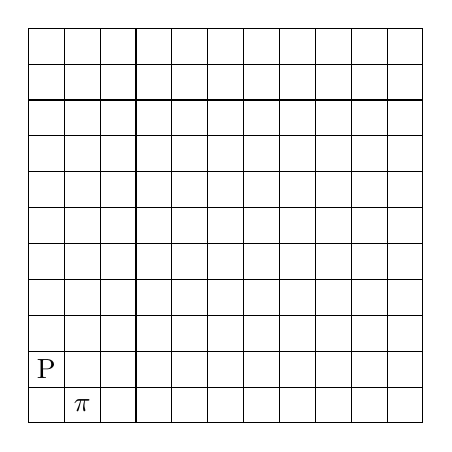
\begin{tikzpicture}
\node [smallgrid] (A) at (0,0) {};
\DrawSmallPrey{1}{2} 
\DrawSmallPred{2}{1}
\end{tikzpicture}
\end{center}
\end{figure}

\section*{Exercise 4}
To find an optimal policy we computed the optimal value function $V^\ast$ for all states in which the prey is located at $\left<5,5\right>$.

The convergence speed (in number of iterations) for different discount factors $\gamma$ is presented in \autoref{tab:convVI}.
\begin{table}
\caption{Trololol.}
\label{tab:convVI}
\begin{center}
\begin{tabular}{|@{ }r@{ }|@{ }r@{ }|}
\hline
Discount factor $\gamma$ & Number of iterations \\
           \hline
0.1 & \\
0.5 & \\
0.7 & \\
0.9 & \\
\hline
\end{tabular}
\end{center}
\end{table}

\section*{Exercise 5}
To iteratively improve the policy we implemented policy iteration $V^{\pi^\prime}$ for all states which the prey is located at $\left<5,5\right>$.

The convergence speed (in number of iterations) for different discount factors $\gamma$ is presented in \autoref{tab:convPI}.
\begin{table}
\caption{Trololol.}
\label{tab:convPI}
\begin{center}
\begin{tabular}{|@{ }r@{ }|@{ }r@{ }|}
\hline
Discount factor $\gamma$ & Number of iterations \\
\hline
0.1 & \\
0.5 & \\
0.7 & \\
0.9 & \\
\hline
\end{tabular}
\end{center}
\end{table}

% TODO: COMPARE THE RESULTS


\newpage
\begin{figure}
\begin{center}
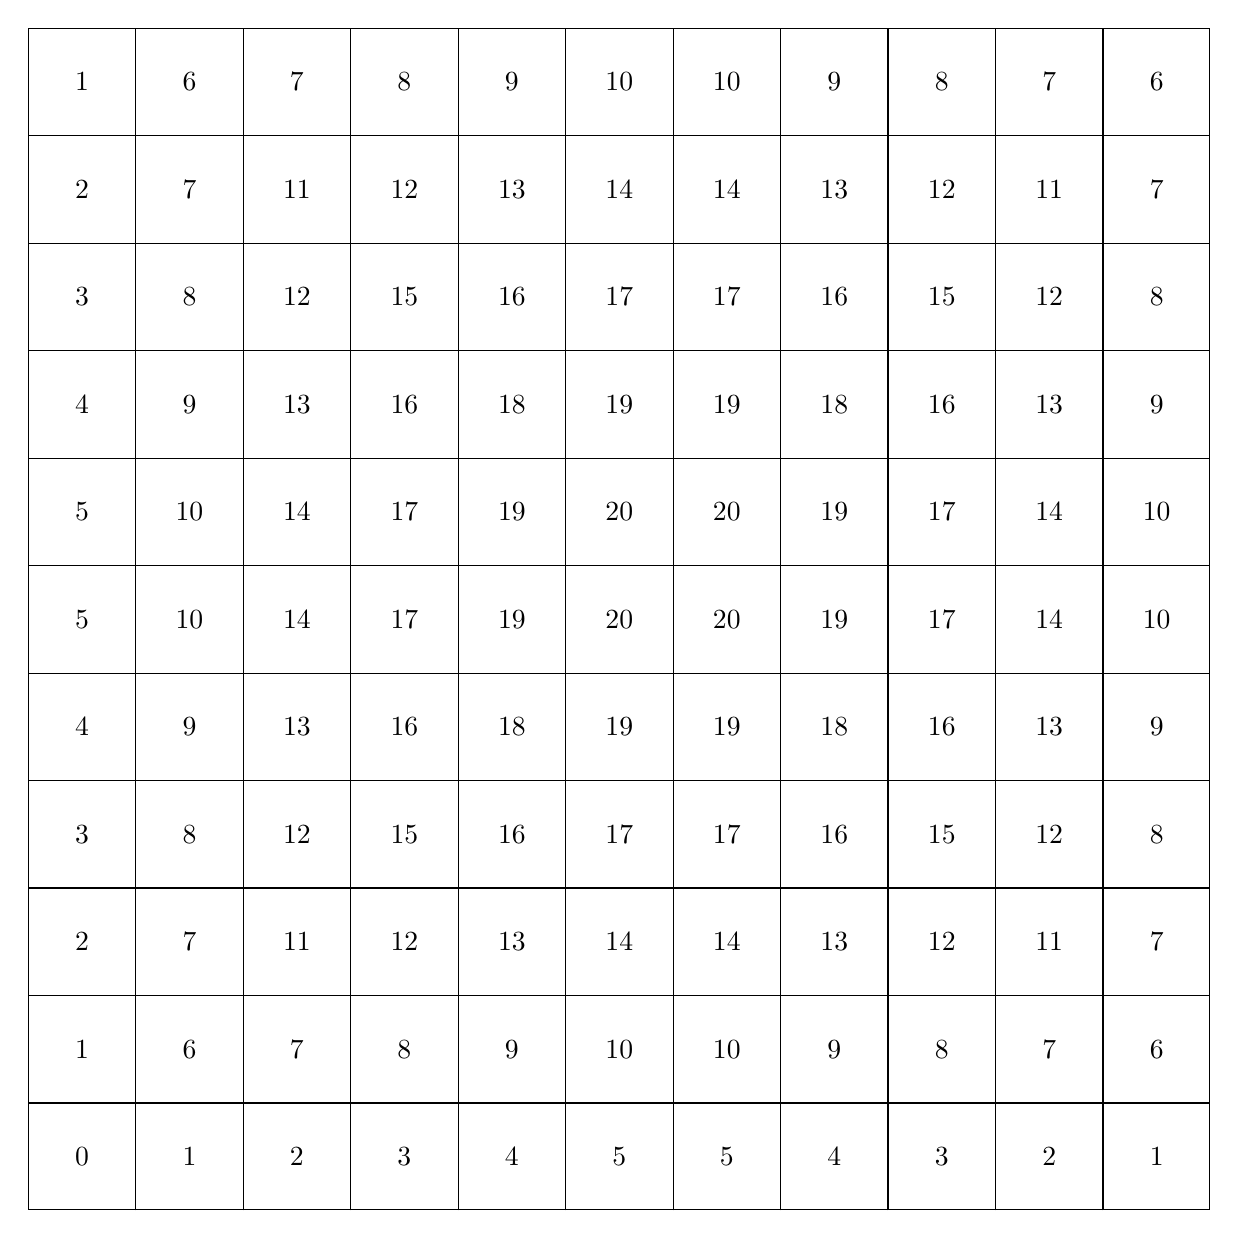
\begin{tikzpicture}
\node[biggrid] (A) at (0,0) {};
\node at (A.center 1  1) {0};
\node at (A.center 2  1) {1};
\node at (A.center 3  1) {2};
\node at (A.center 4  1) {3};
\node at (A.center 5  1) {4};
\node at (A.center 6  1) {5};
\node at (A.center 7  1) {5};
\node at (A.center 8  1) {4};
\node at (A.center 9  1) {3};
\node at (A.center 10 1) {2};
\node at (A.center 11 1) {1};
\node at (A.center 1  2) {1};
\node at (A.center 2  2) {6};
\node at (A.center 3  2) {7};
\node at (A.center 4  2) {8};
\node at (A.center 5  2) {9};
\node at (A.center 6  2) {10};
\node at (A.center 7  2) {10};
\node at (A.center 8  2) {9};
\node at (A.center 9  2) {8};
\node at (A.center 10 2) {7};
\node at (A.center 11 2) {6};
\node at (A.center 1  3) {2};
\node at (A.center 2  3) {7};
\node at (A.center 3  3) {11};
\node at (A.center 4  3) {12};
\node at (A.center 5  3) {13};
\node at (A.center 6  3) {14};
\node at (A.center 7  3) {14};
\node at (A.center 8  3) {13};
\node at (A.center 9  3) {12};
\node at (A.center 10 3) {11};
\node at (A.center 11 3) {7};
\node at (A.center 1  4) {3};
\node at (A.center 2  4) {8};
\node at (A.center 3  4) {12};
\node at (A.center 4  4) {15};
\node at (A.center 5  4) {16};
\node at (A.center 6  4) {17};
\node at (A.center 7  4) {17};
\node at (A.center 8  4) {16};
\node at (A.center 9  4) {15};
\node at (A.center 10 4) {12};
\node at (A.center 11 4) {8};
\node at (A.center 1  5) {4};
\node at (A.center 2  5) {9};
\node at (A.center 3  5) {13};
\node at (A.center 4  5) {16};
\node at (A.center 5  5) {18};
\node at (A.center 6  5) {19};
\node at (A.center 7  5) {19};
\node at (A.center 8  5) {18};
\node at (A.center 9  5) {16};
\node at (A.center 10 5) {13};
\node at (A.center 11 5) {9};
\node at (A.center 1  6) {5};
\node at (A.center 2  6) {10};
\node at (A.center 3  6) {14};
\node at (A.center 4  6) {17};
\node at (A.center 5  6) {19};
\node at (A.center 6  6) {20};
\node at (A.center 7  6) {20};
\node at (A.center 8  6) {19};
\node at (A.center 9  6) {17};
\node at (A.center 10 6) {14};
\node at (A.center 11 6) {10};
\node at (A.center 1  11) {1};
\node at (A.center 2  11) {6};
\node at (A.center 3  11) {7};
\node at (A.center 4  11) {8};
\node at (A.center 5  11) {9};
\node at (A.center 6  11) {10};
\node at (A.center 7  11) {10};
\node at (A.center 8  11) {9};
\node at (A.center 9  11) {8};
\node at (A.center 10 11) {7};
\node at (A.center 11 11) {6};
\node at (A.center 1  10) {2};
\node at (A.center 2  10) {7};
\node at (A.center 3  10) {11};
\node at (A.center 4  10) {12};
\node at (A.center 5  10) {13};
\node at (A.center 6  10) {14};
\node at (A.center 7  10) {14};
\node at (A.center 8  10) {13};
\node at (A.center 9  10) {12};
\node at (A.center 10 10) {11};
\node at (A.center 11 10) {7};
\node at (A.center 1  9) {3};
\node at (A.center 2  9) {8};
\node at (A.center 3  9) {12};
\node at (A.center 4  9) {15};
\node at (A.center 5  9) {16};
\node at (A.center 6  9) {17};
\node at (A.center 7  9) {17};
\node at (A.center 8  9) {16};
\node at (A.center 9  9) {15};
\node at (A.center 10 9) {12};
\node at (A.center 11 9) {8};
\node at (A.center 1  8) {4};
\node at (A.center 2  8) {9};
\node at (A.center 3  8) {13};
\node at (A.center 4  8) {16};
\node at (A.center 5  8) {18};
\node at (A.center 6  8) {19};
\node at (A.center 7  8) {19};
\node at (A.center 8  8) {18};
\node at (A.center 9  8) {16};
\node at (A.center 10 8) {13};
\node at (A.center 11 8) {9};
\node at (A.center 1  7) {5};
\node at (A.center 2  7) {10};
\node at (A.center 3  7) {14};
\node at (A.center 4  7) {17};
\node at (A.center 5  7) {19};
\node at (A.center 6  7) {20};
\node at (A.center 7  7) {20};
\node at (A.center 8  7) {19};
\node at (A.center 9  7) {17};
\node at (A.center 10 7) {14};
\node at (A.center 11 7) {10};
\end{tikzpicture}
\end{center}
\end{figure}
\end{document}

